Испытания представляют собой процесс установления соответствия программы и
программной документации заданным требованиям.

\subsubsection{Проверка требований к документации}
Проверяеться наличие всех документов перечисленных в пyнкте 4.1 данного документа и их соответствие ГОСТ.

\subsection{Проверка требований к интерфейсу}
Интерфейс соответствует схеме, указанной в техническом задании. Совместим а ОС Андроид. Имеет в центре экрана reticle  и полосу загрузки (слайдер) внизу. Цветовая палитра взята с сайта, указанного в настоящем Техническом Задании.

\begin{figure}[h!]
    \centering
    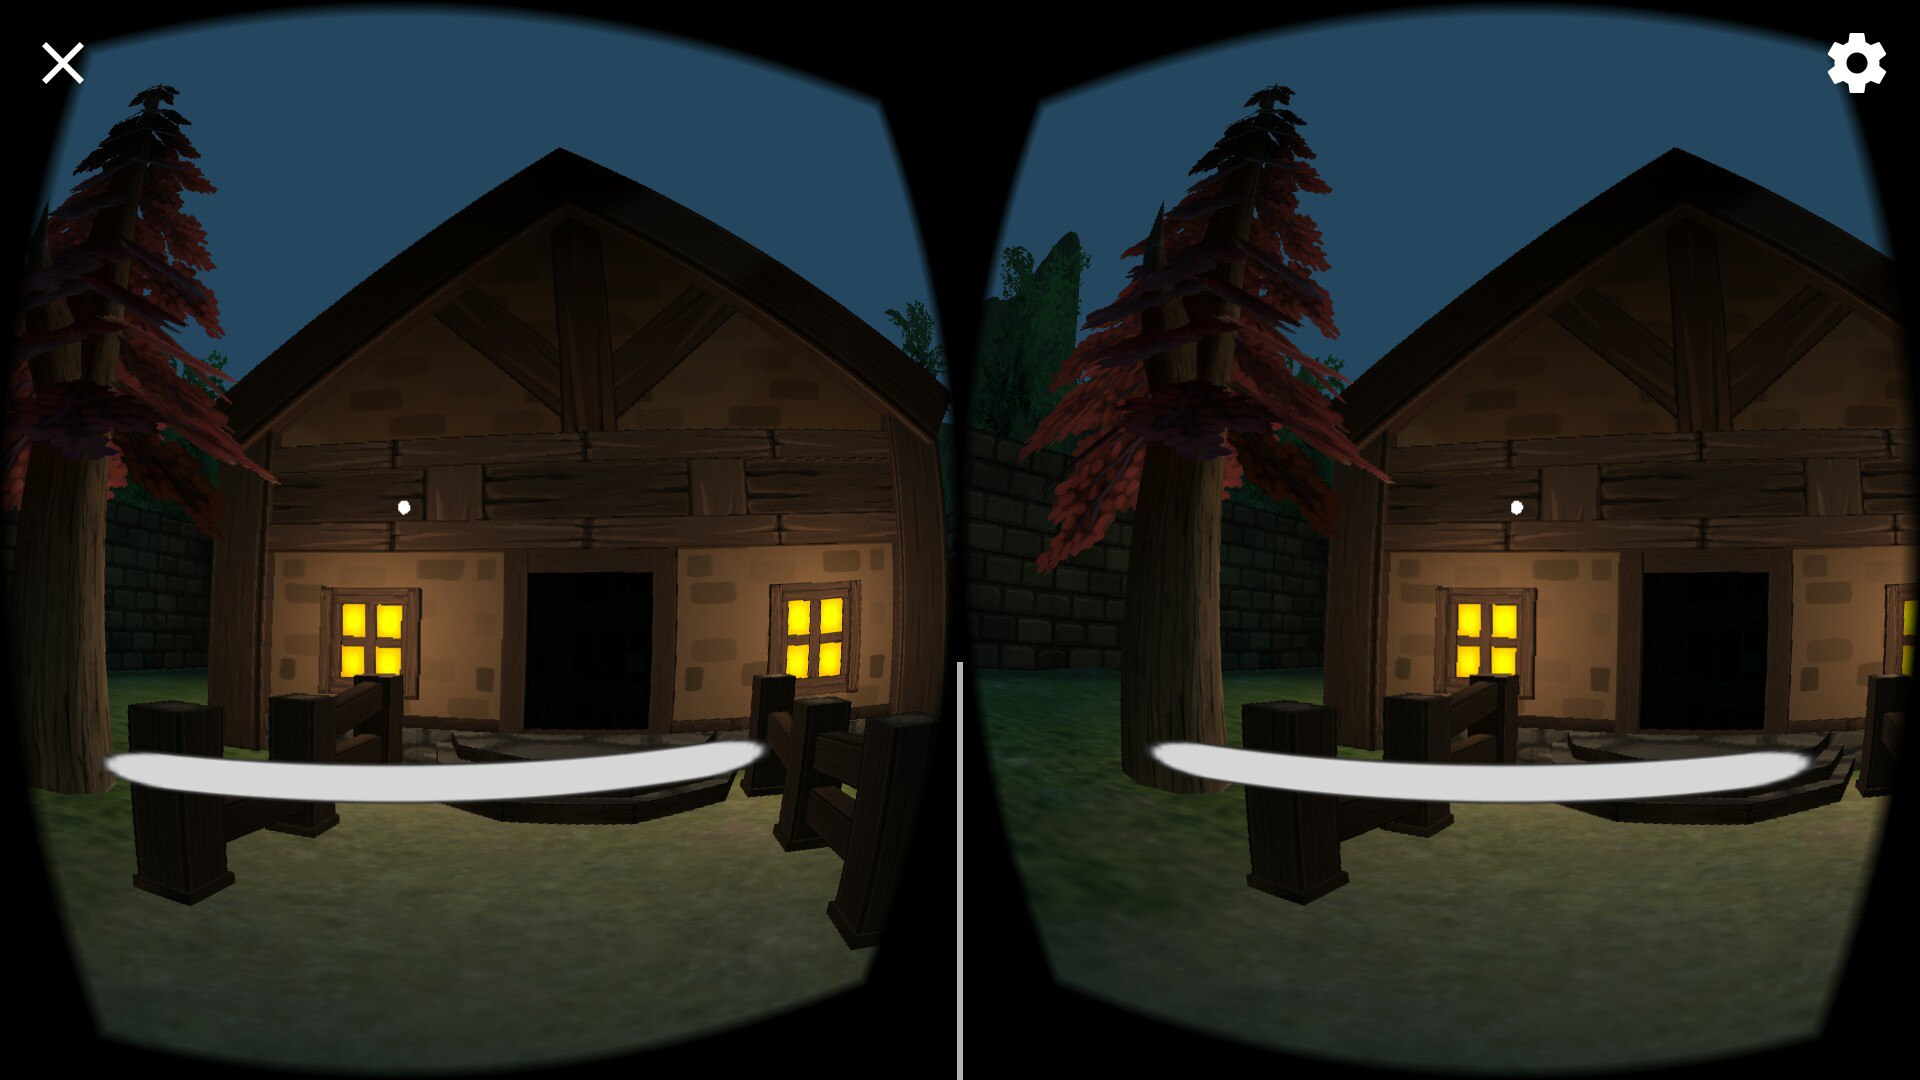
\includegraphics[width=0.7\textwidth]{./screenshots/home.jpg}
    \caption{проверка требований к интерфейсу}
    \label{home}
\end{figure}

\newpage
\subsection{Проверка требований к функциональным характеристикам}

Запуск игры в режиме VR Mode и Normal Mode присутствует. Передвижение персонажа осуществляется в скрипте WalkByLook.cs при помощи углов наклона головы относительно оси Х, без нажатия триггера.

\begin{figure}[h!]
    \centering
    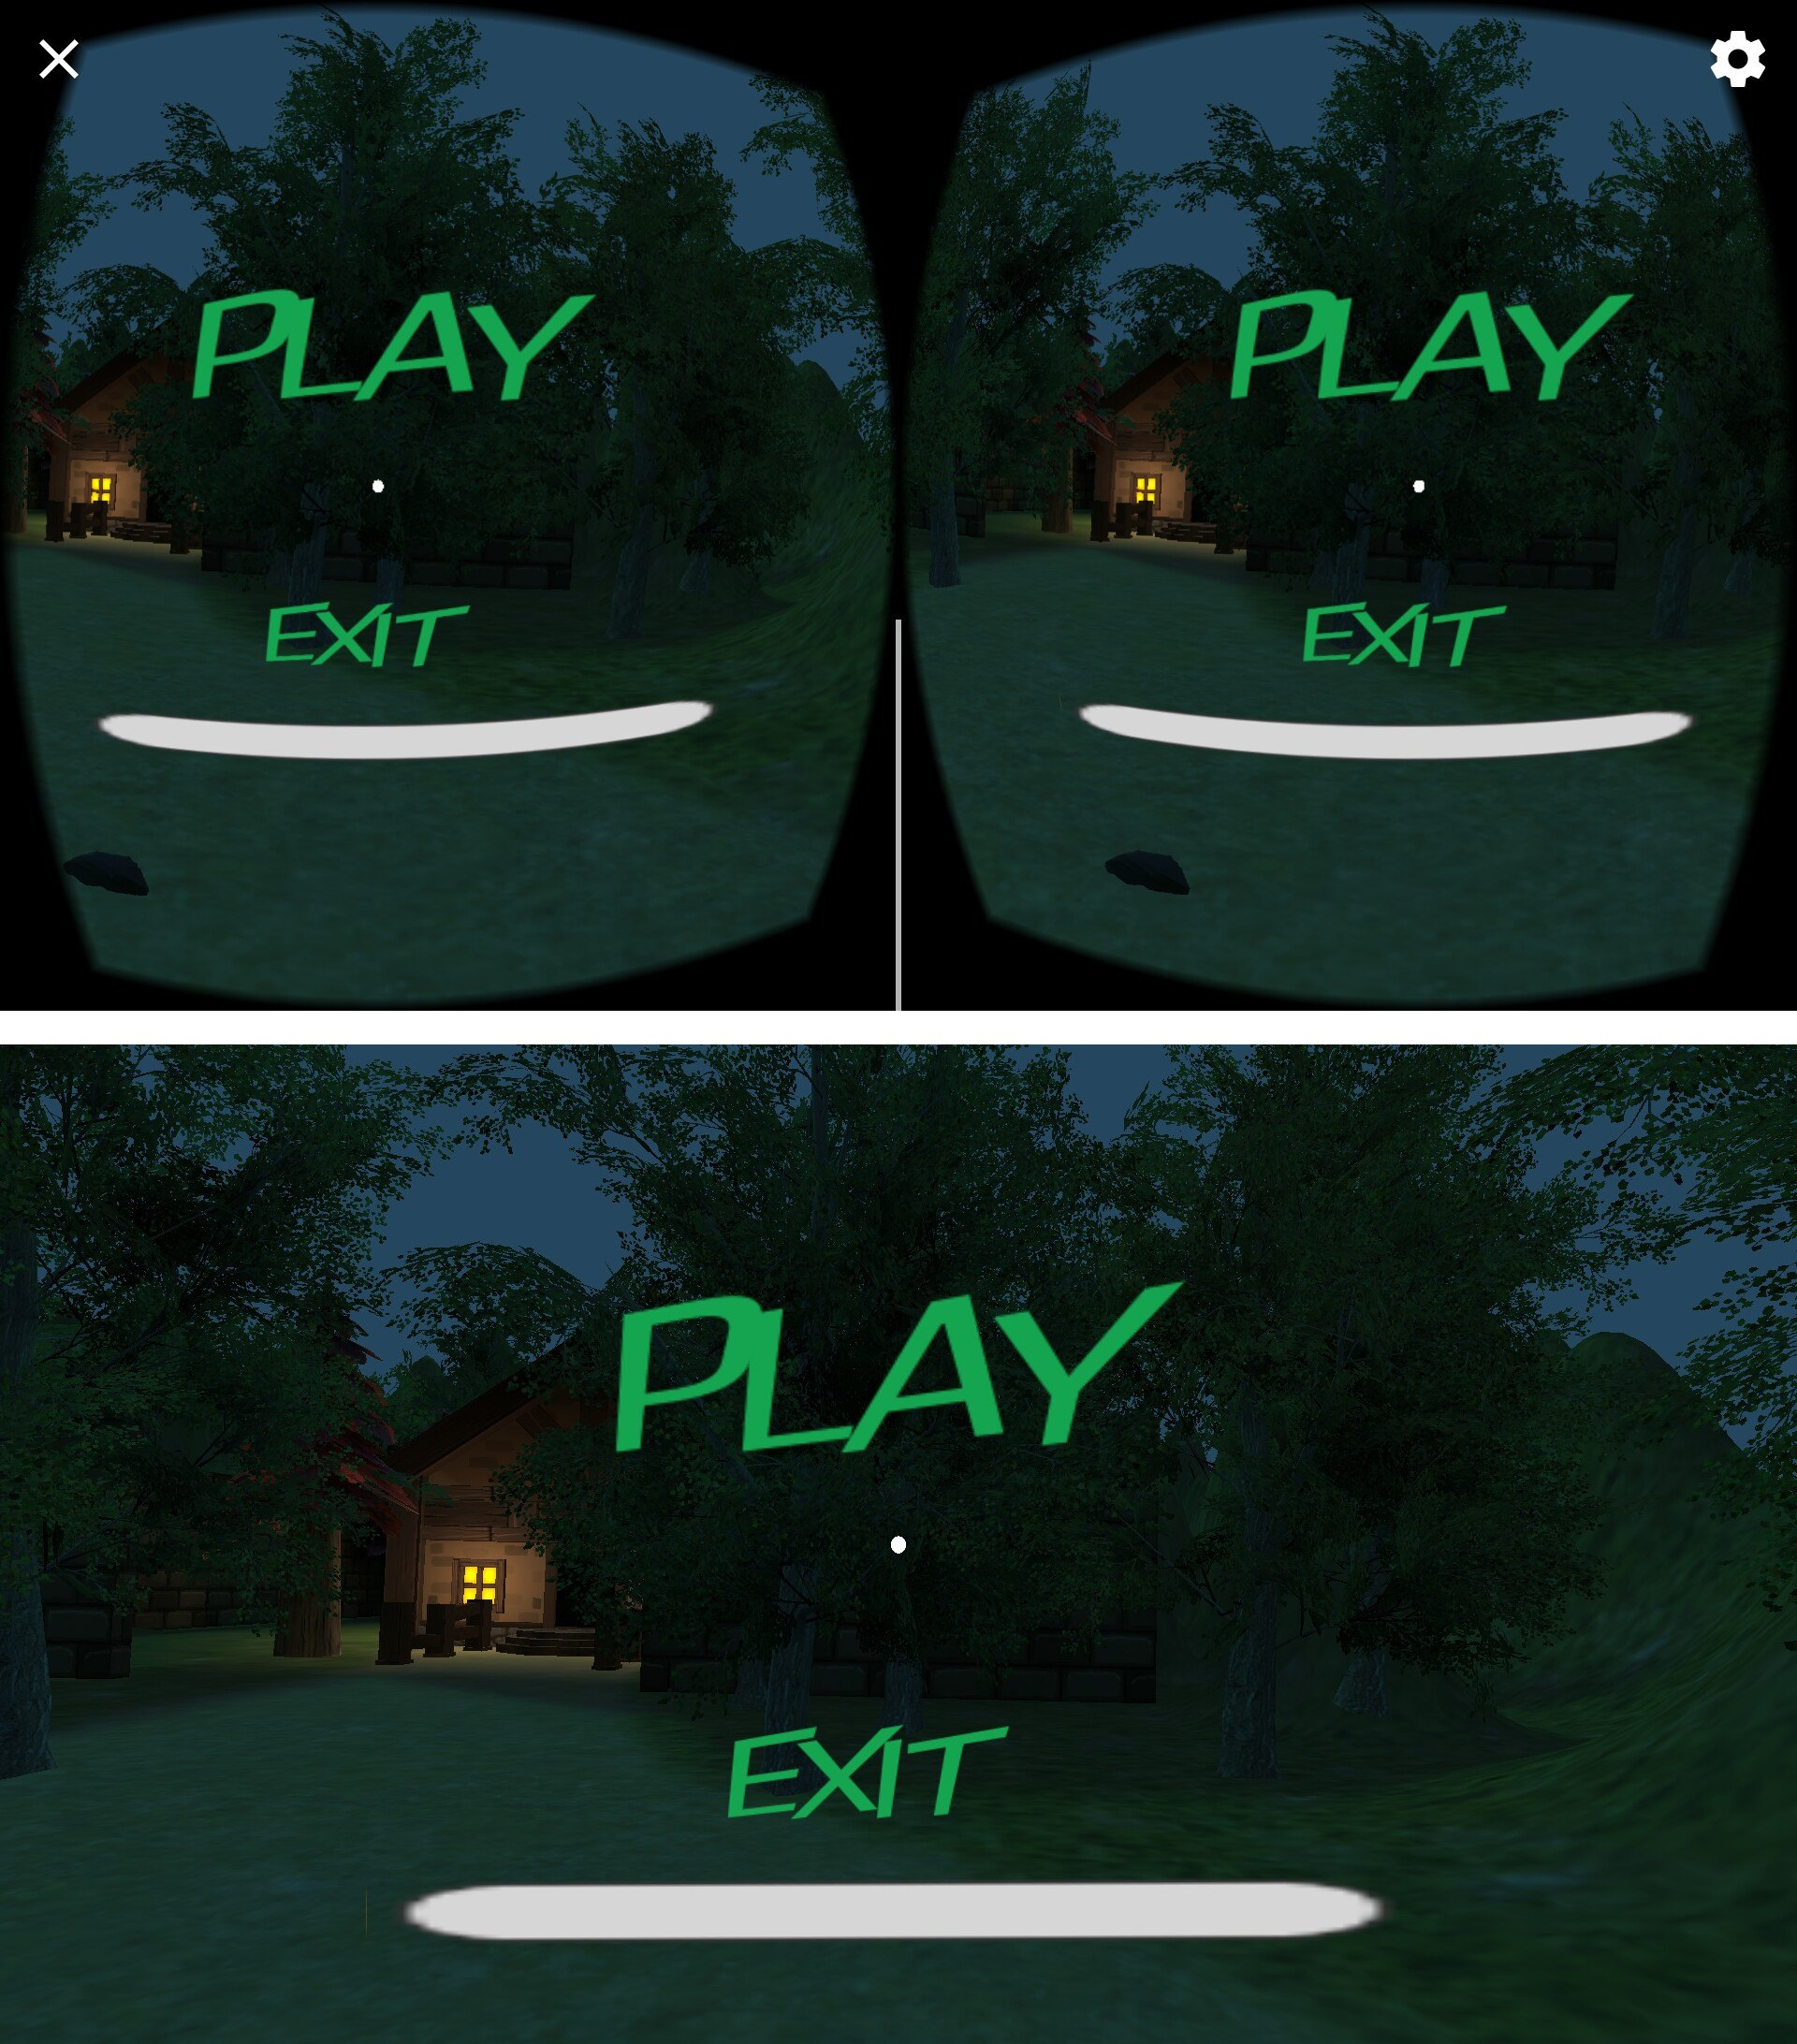
\includegraphics[width=0.7\textwidth]{./screenshots/diff.jpg}
    \caption{разница между VR Mode и Normal Mode}
    \label{diff}
\end{figure}

\begin{figure}[h!]
    \centering
    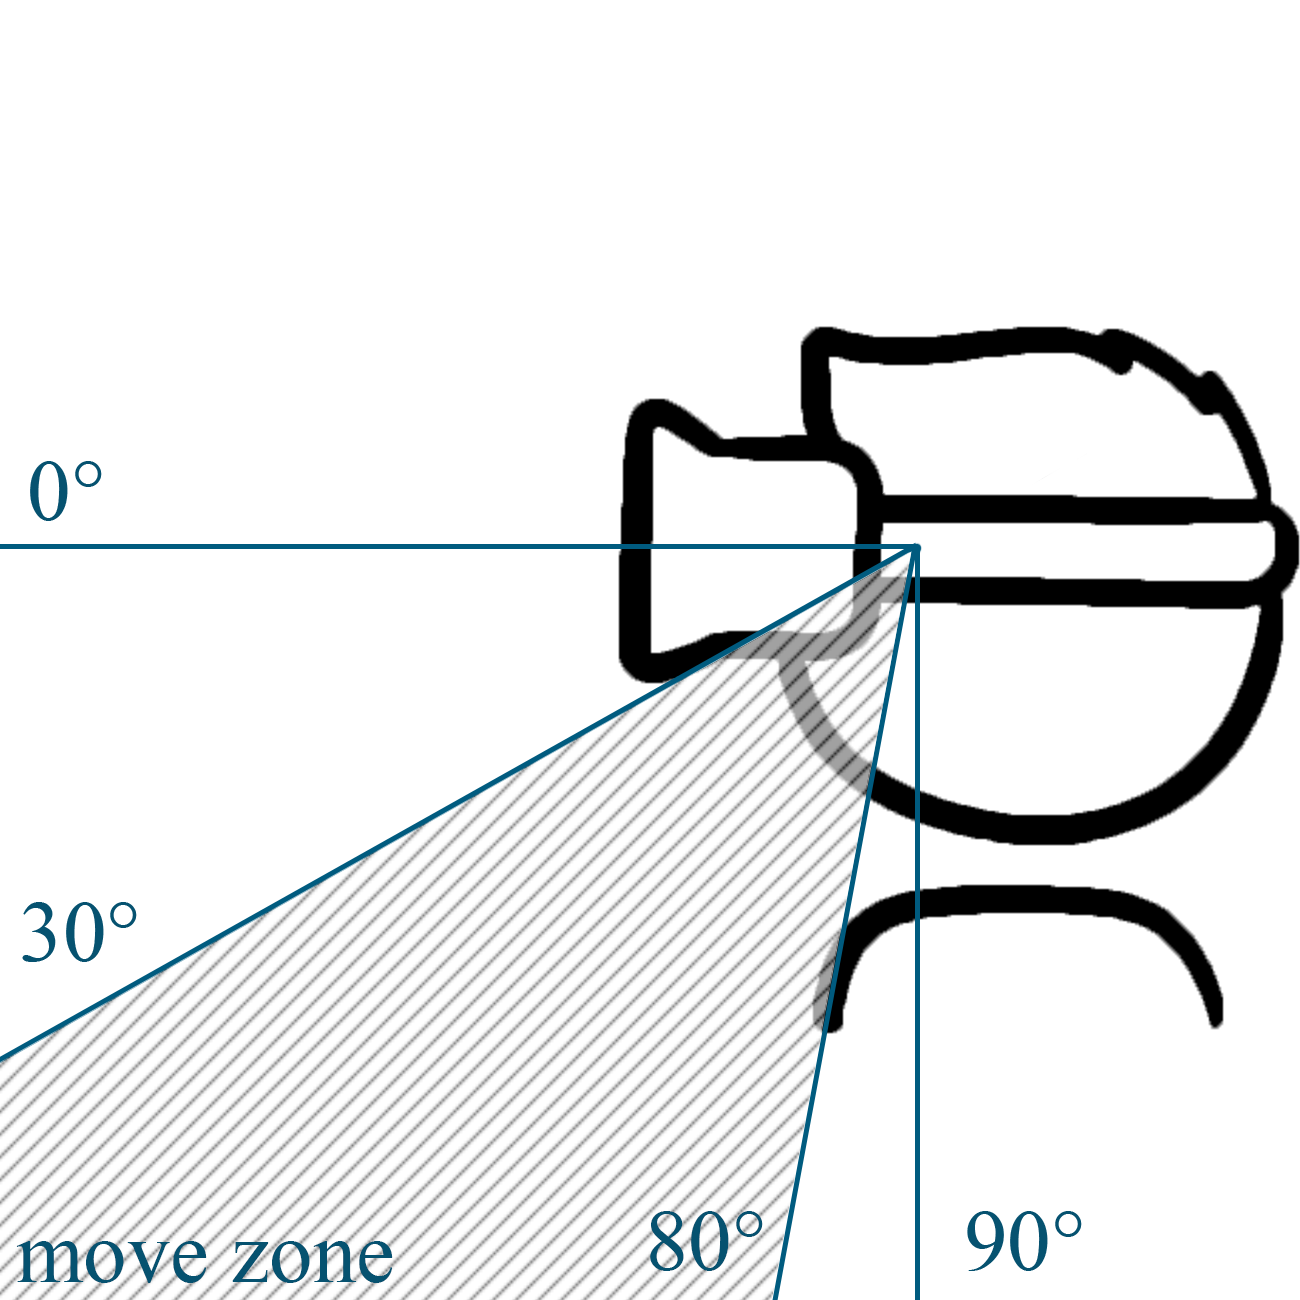
\includegraphics[width=0.7\textwidth]{./pics/vrAngles.png}
    \caption{схема передвижения в данной игре}
    \label{angles}
\end{figure}

Предметы можно поднимать и бросать без нажатия триггера - за это отвечает скрипт PickUpObject.cs.

\begin{figure}[h!]
    \centering
    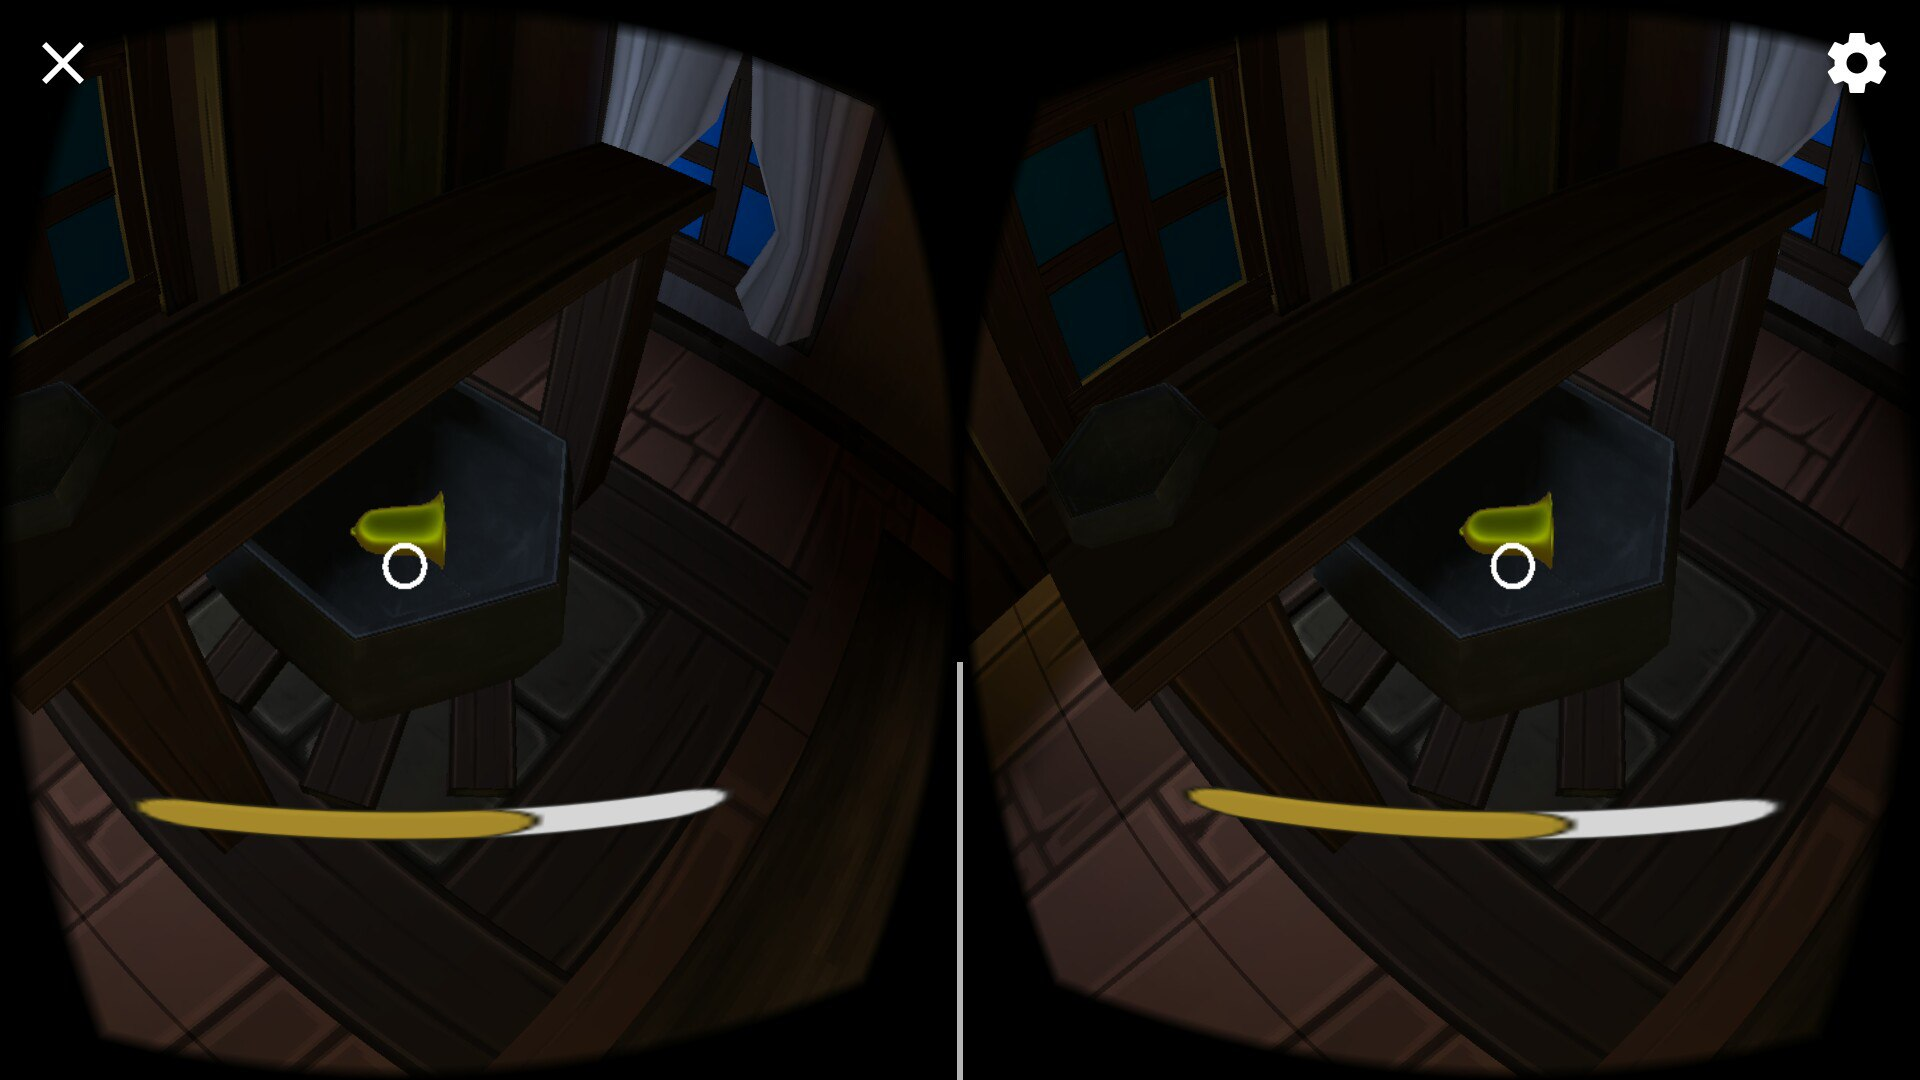
\includegraphics[width=0.7\textwidth]{./screenshots/pick_up_bell.jpg}
    \caption{поднятие предмета}
    \label{pick_up}
\end{figure}

Отображение пользователю актуальной на данный момент времени информации.

\begin{figure}[h!]
    \centering
    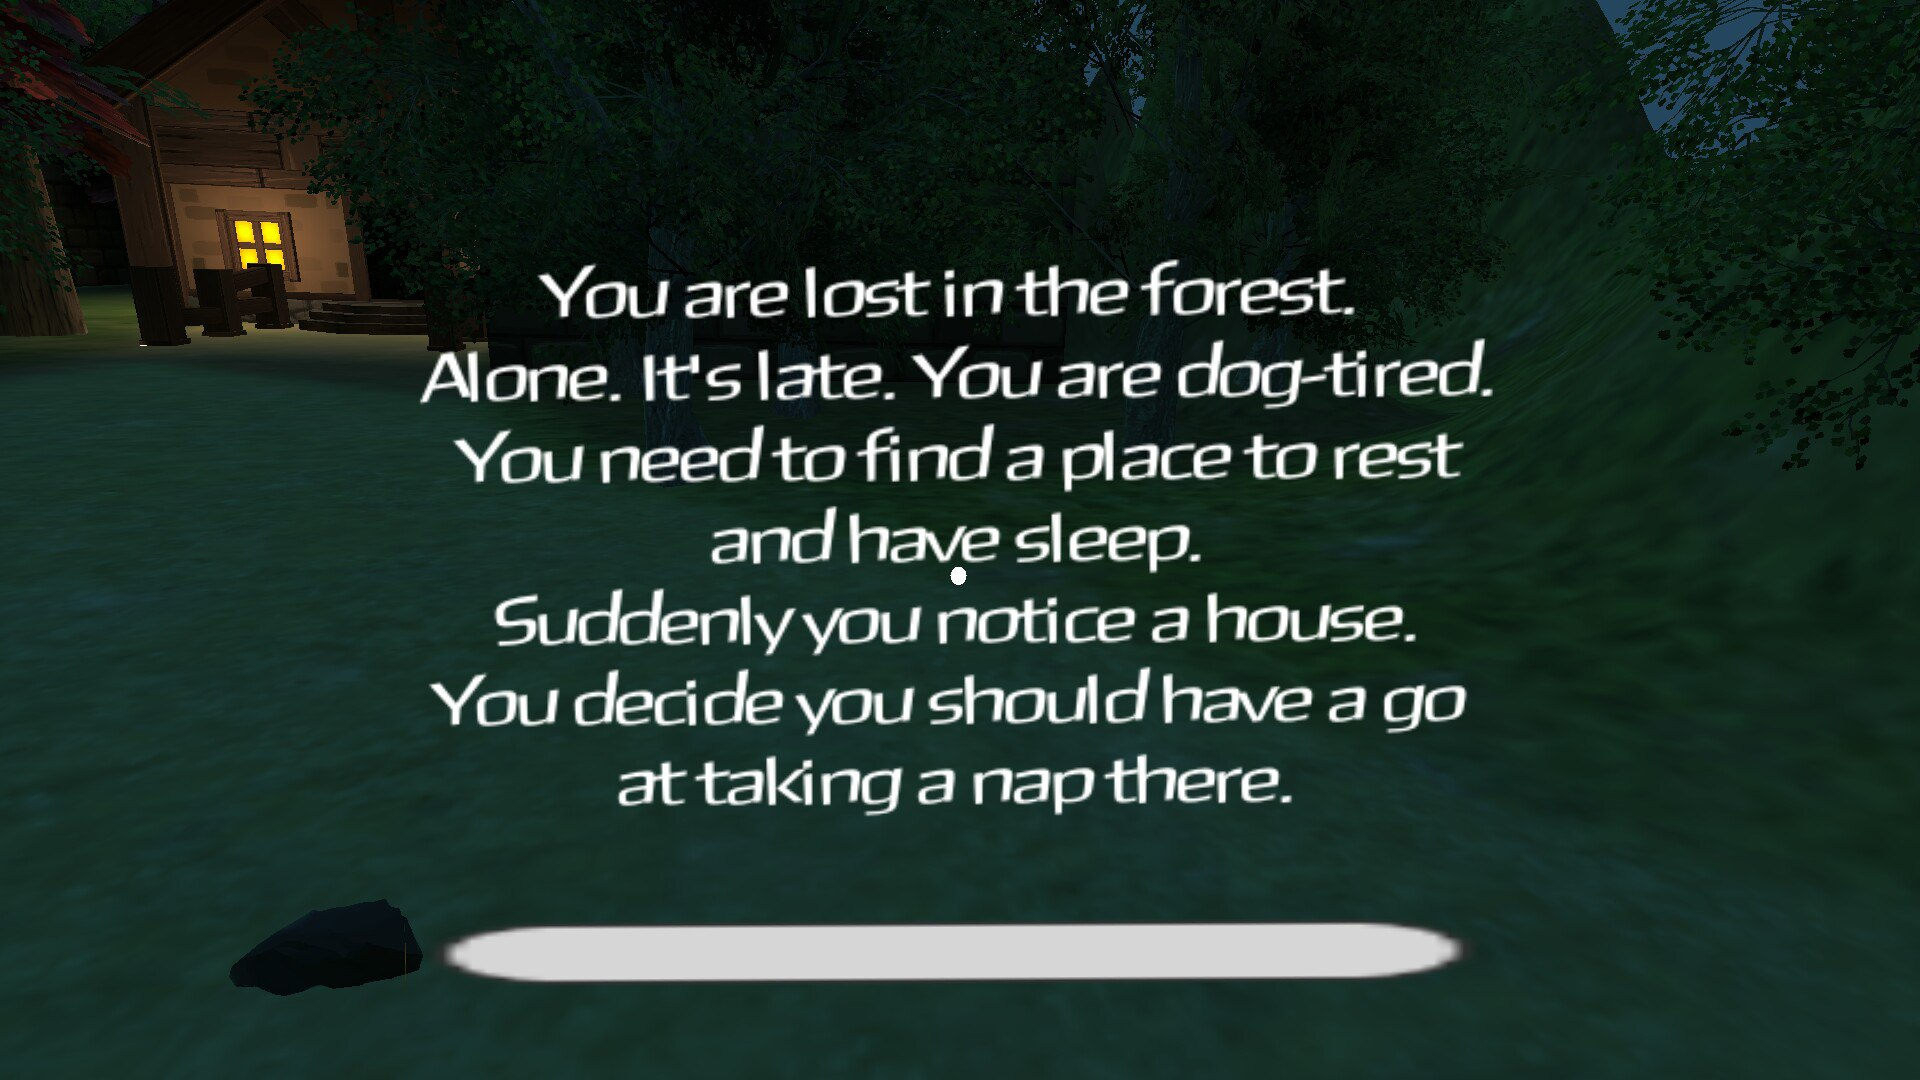
\includegraphics[width=0.7\textwidth]{./screenshots/info_normal.jpg}
    \caption{Начальная информация (снимок сделан в Normal Mode, для разнообразия)}
    \label{info_normal}
\end{figure}

Начало показа обучающего фрагмента. Реализовано обучение в начале игры.

\begin{figure}[h!]
    \centering
    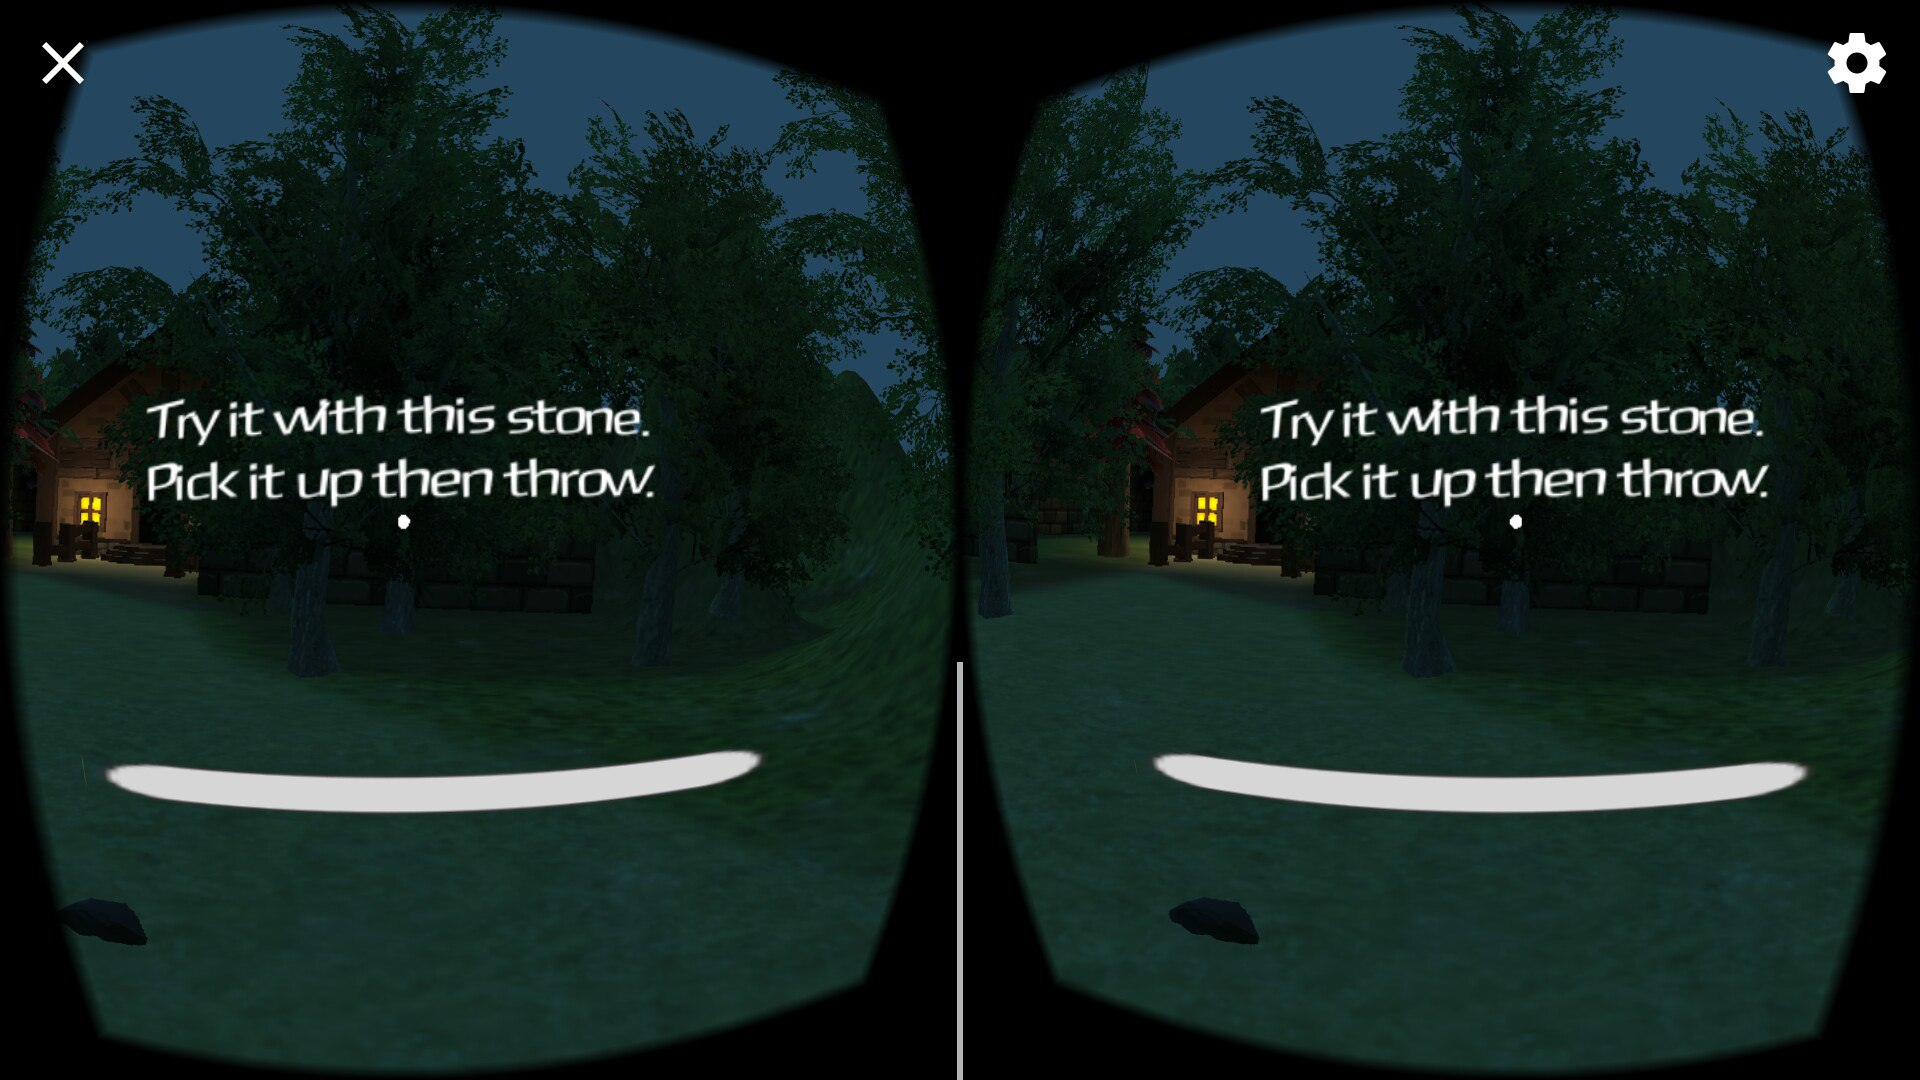
\includegraphics[width=0.7\textwidth]{./screenshots/try.jpg}
    \caption{Приглашение попробовать взять и кинуть камень}
    \label{try}
\end{figure}













\newpage
\subsection{Проверка требований к временным характеристикам}
Все временные характеристики соблюдены (рис. \ref{stats})
\begin{figure}[h!]
    \centering
    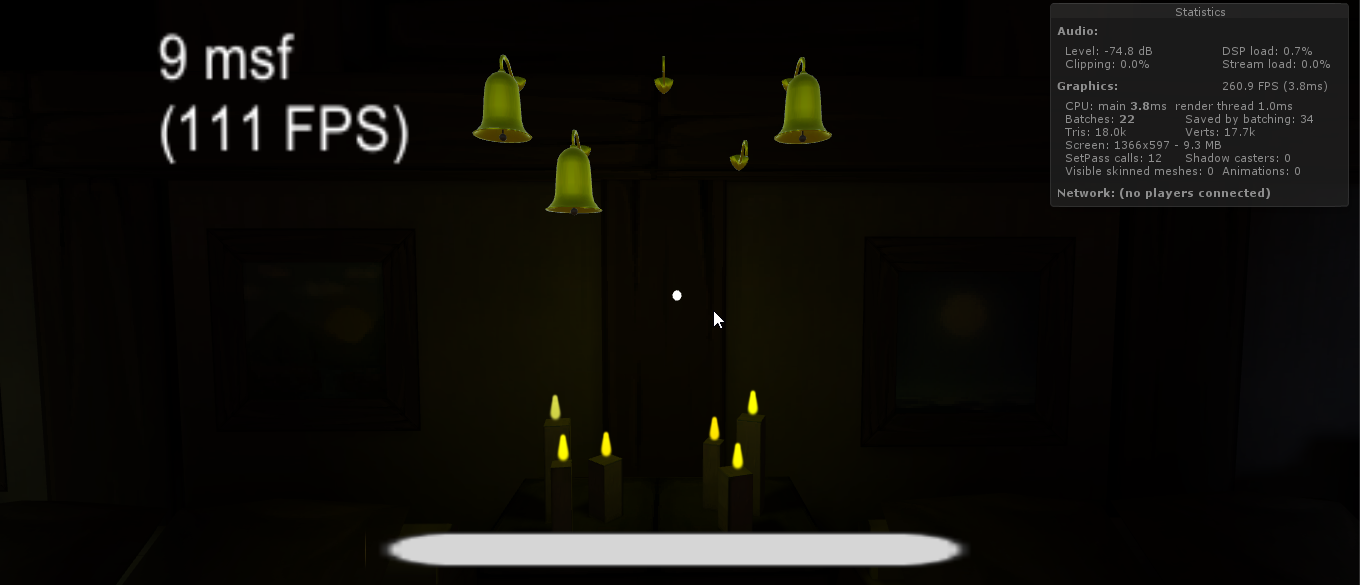
\includegraphics[width=0.8\textwidth]{./screenshots/stats.png}
    \caption{статистика для проверки временных характеристик}
    \label{stats}
\end{figure}



